\documentclass[conference]{IEEEtran}
\IEEEoverridecommandlockouts
\usepackage{cite}
\usepackage{amsmath,amssymb,amsfonts,amsthm}
\usepackage{algorithm}
\usepackage{algorithmic}
\usepackage{graphicx}
\usepackage{booktabs}
\usepackage{textcomp}
\usepackage{xcolor}
\usepackage{tikz}
\usetikzlibrary{positioning,arrows.meta}
\usepackage[hidelinks]{hyperref}
\newtheorem{proposition}{Proposition}

\begin{document}

\title{IMBANG: Balancing DDoS Mitigation and Service Outages with Safety-Spanning Group-Relative Policy Optimisation}

\author{\IEEEauthorblockN{Author One\IEEEauthorrefmark{1}, Author Two\IEEEauthorrefmark{1}, and Author Three\IEEEauthorrefmark{2}}
\IEEEauthorblockA{\IEEEauthorrefmark{1}Affiliation, City, Country\\
\IEEEauthorrefmark{2}Affiliation, City, Country\\
Email: \{author1, author2\}@institution.edu, author3@institution.edu}}

\maketitle

\begin{abstract}
A DDoS controller at the 6G edge is useful only if it removes attack traffic without starving legitimate users. Sentinel, a recent neuro-symbolic mitigation framework, trains a shielded PPO agent against a co-evolving attacker. By its own account, that training deteriorates late in every run, and severe outages persist under heavy floods. Replacing co-evolution with critic-free Group Relative Policy Optimization (GRPO) removes the value network and the learned opponent. We show that it also introduces a new hazard. A penalty that every rollout in a group incurs cancels out of the group-normalised advantage, so the outage constraint vanishes whenever sampled actions stop straddling the outage boundary, and the leakage gradient drives the policy across it. Across 80 trained checkpoints, the share of groups that straddle the boundary follows the spread of the sampled actions ($r=0.91$) and moves against the severe-outage rate ($r=-0.61$). IMBANG restores the missing signal by adding one \emph{safe-side member} to each group. This member replays the policy's own action, shifted in a direction that provably cannot raise collateral damage. An outage budget enforced through a Lagrange multiplier and a discrete minimax-regret curriculum complete the method. Over ten seeds, IMBANG outscores Sentinel's published checkpoints in all eight attack scenarios after Holm correction. It lowers severe outages from 34.4 to 14.8 per 500 control steps, raises the red-team worst case from $-1.07$ to $-0.72$, and satisfies the outage budget in nine seeds out of ten, against three for Constrained GRPO. IMBANG also outperforms a compute-matched PPO baseline, and its deployed policy takes under 0.3\,ms per decision on a single CPU core.
\end{abstract}

\begin{IEEEkeywords}
6G security, DDoS mitigation, safe reinforcement learning, group-relative policy optimisation, zero-touch network management.
\end{IEEEkeywords}

% ===========================================================================
\section{Introduction}
% ===========================================================================
Zero-touch management is expected to let 6G networks defend themselves in closed loop, with the operator supervising rather than intervening~\cite{benzaid2020zsm,liyanage2023oran}. Volumetric DDoS attacks make this difficult. The mitigation controller must discard as much hostile traffic as possible, yet every legitimate packet it discards is itself a service failure. An over-eager filter can therefore cause the very outage it was deployed to prevent, and operators need to see why a filter acted as it did~\cite{guo2020xai6g,senevirathna2025xaib5gsec}.

Deep reinforcement learning (DRL) has been applied to router throttling, SDN flow control and per-host drop policies~\cite{malialis2015distributed,liu2018drlddos,simpson2020perhost,akbari2020atmos}. The most complete recent design, Sentinel~\cite{alfatemi2026sentinel}, trains its agent with Proximal Policy Optimization (PPO)~\cite{schulman2017ppo} and places a symbolic runtime shield~\cite{alshiekh2018shielding} between that agent and the network. It trains that defender against a learned attacker with a Hall-of-Fame opponent archive and distils the result into shallow decision trees. Sentinel's authors report three weaknesses openly. Its training deteriorates late in all ten seeds. Outside the held-out ICMP scenario, the shielded policy performs like its unshielded ablation. And severe outages remain common under high-rate floods.

GRPO~\cite{shao2024deepseekmath} appears to address the first weakness naturally. It estimates advantages by comparing several rollouts that start from the same state, so no value network is needed. In a simulator, these rollouts can share one realisation of the traffic process (common random numbers~\cite{ng2000pegasus}), leaving the defender's actions as the only difference between them. Our first finding is less welcome. GRPO defenders block more attack traffic than Sentinel, but they also cause \emph{more} severe outages than Sentinel or an equally trained PPO baseline. We trace this to a structural property of group-relative training. A cost shared by all members of a group is removed by the group mean, just as a binary reward that is identical across a group yields no gradient~\cite{nie2026starvation,yu2025dapo}. Once the sampled actions all sit on the same side of the outage boundary, the outage constraint exerts no pull at all.

\textbf{Contributions.} The paper explains \emph{why} critic-free training makes DDoS defenders unsafe and shows how to prevent it. It makes three contributions.
\begin{itemize}
\item \emph{Diagnosis.} We identify and formalise the \emph{constraint-cancellation} effect: group-relative updates lose any safety cost that a whole group shares (Prop.~\ref{prop:cancel}). We confirm it on 80 trained checkpoints (Section~\ref{sec:mechanism}).
\item \emph{Remedy with a guarantee.} IMBANG (Malay for \emph{balance}) keeps every group straddling the outage boundary through a \emph{safe-side member}: the policy's own sample moved along a direction that, by the service model and the shield, cannot be less safe (Prop.~\ref{prop:safe}). It adds a Lagrangian outage budget and a discrete minimax-regret curriculum. The deployed policy has only 5.4k parameters and decides in under 0.3\,ms on one CPU core (Section~\ref{sec:method}).
\item \emph{Evidence.} We compare IMBANG against Sentinel's own ten released checkpoints, a compute-matched PPO baseline, Constrained GRPO~\cite{girgis2026cgrpo} and the simplest alternative remedies. The evaluation runs on a test-verified port of Sentinel's simulator, under three protocols with paired statistical tests (Section~\ref{sec:eval}).
\end{itemize}

% ===========================================================================
\section{Related Work}
% ===========================================================================
\textbf{Learning-based DDoS defence.} Detection models such as LUCID~\cite{doriguzzi2020lucid} label traffic but leave the choice of countermeasure to others. Control-oriented work learns throttling rates~\cite{malialis2015distributed}, OpenFlow reconfiguration~\cite{liu2018drlddos,akbari2020atmos} or per-host drop probabilities~\cite{simpson2020perhost}. Sentinel~\cite{alfatemi2026sentinel} adds runtime shielding, adversarial co-evolution and tree extraction; it is the reference system we aim to surpass. In 6G security, GRPO has so far been used to tune a language-model strategy generator for zero-touch networks~\cite{cao2025secloop}, not a numerical mitigation policy.

\textbf{Critic-free and constrained optimisation.} GRPO~\cite{shao2024deepseekmath,guo2025deepseekr1} substitutes a group average for the learned baseline of actor-critic methods~\cite{schulman2016gae}. Several of its pathologies have been examined in language-model training: length and normalisation bias, entropy collapse, and groups with no reward variance~\cite{liu2025understanding,yu2025dapo,nie2026starvation}. Its performance on classical control has also been questioned~\cite{oliveira2025critics,wang2026gr2po}. Constrained RL enforces safety either by restricting policy updates~\cite{achiam2017cpo} or through Lagrange multipliers. Constrained GRPO~\cite{girgis2026cgrpo} normalises the reward and cost channels separately before mixing them. As shown below, however, a separately normalised cost still carries no information when it does not vary inside a group. Adding reference samples to GRPO groups is known to stabilise language-model training~\cite{yan2025luffy,armor2026}. Our safe-side member differs because it is built from the policy's own sample along a known monotone safety direction, and it exists only to create cost variation. For the training distribution we draw on regret-based curricula~\cite{dennis2020paired,jiang2021plr,parkerholder2022accel,rutherford2024noregrets}, using the MaxMC regret estimate of~\cite{jiang2021robustplr} over a discrete set of attack levels. Table~\ref{tab:related} contrasts these approaches.

\begin{table}[t]
\centering
\caption{Positioning Against the Closest Approaches}
\label{tab:related}
\setlength{\tabcolsep}{2.5pt}
\resizebox{\columnwidth}{!}{%
\begin{tabular}{@{}lcccc@{}}
\toprule
 & Critic- & No learned & Outage & Cost signal when all \\
Approach & free & attacker & budget & members violate \\
\midrule
Sentinel~\cite{alfatemi2026sentinel} & -- & -- & -- & n/a (critic) \\
PPO-Lagrangian / CPO~\cite{achiam2017cpo} & -- & \checkmark & \checkmark & n/a (critic) \\
GRPO~\cite{shao2024deepseekmath} with penalty & \checkmark & \checkmark & \checkmark & -- \\
Constrained GRPO~\cite{girgis2026cgrpo} & \checkmark & \checkmark & \checkmark & -- \\
Sign advantage~\cite{nie2026starvation} & \checkmark & \checkmark & -- & fixed reference \\
\textbf{IMBANG (ours)} & \checkmark & \checkmark & \checkmark & \checkmark\ (safe member) \\
\bottomrule
\end{tabular}}
\end{table}

% ===========================================================================
\section{System Model and Problem Formulation}
\label{sec:model}
% ===========================================================================
\begin{figure}[t]
\centering
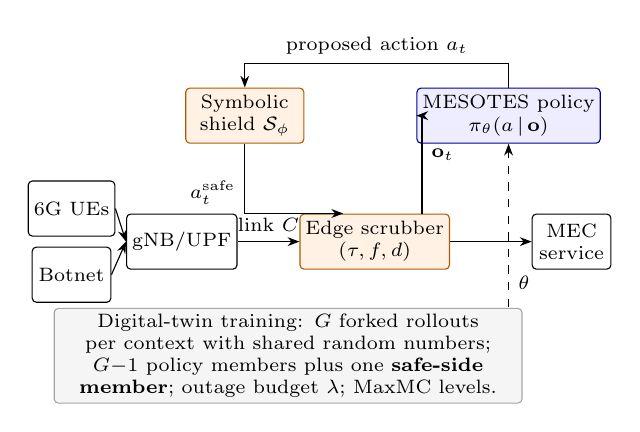
\begin{tikzpicture}[font=\scriptsize, >={Stealth[length=1.5mm]},
  box/.style={draw, rounded corners=1.5pt, align=center, inner sep=2pt, minimum height=7mm, fill=white},
  ag/.style={box, fill=blue!7, draw=blue!60!black}, sy/.style={box, fill=orange!10, draw=orange!70!black},
  tr/.style={box, fill=gray!8, draw=gray!70}]
\node[box, minimum width=10mm] (ue) at (0, 0.42) {6G UEs};
\node[box, minimum width=10mm] (bot) at (0,-0.42) {Botnet};
\node[box, minimum width=11mm] (gnb) at (1.4, 0) {gNB/UPF};
\node[sy, minimum width=17mm] (scr) at (3.85, 0) {Edge scrubber\\$(\tau,f,d)$};
\node[box, minimum width=10mm] (mec) at (6.35, 0) {MEC\\service};
\node[ag, minimum width=19mm] (pol) at (5.55, 1.6) {MESOTES policy\\$\pi_\theta(a\,|\,\mathbf{o})$};
\node[sy, minimum width=15mm] (sh) at (2.2, 1.6) {Symbolic\\shield $\mathcal{S}_\phi$};
\node[tr, text width=58mm] (twin) at (2.75,-1.45) {Digital-twin training: $G$ forked rollouts per context with shared random numbers; $G{-}1$ policy members plus one \textbf{safe-side member}; outage budget $\lambda$; MaxMC levels.};
\draw[->] (ue.east) -- (gnb.west);
\draw[->] (bot.east) -- (gnb.west);
\draw[->] (gnb) -- node[above]{link $C$} (scr);
\draw[->] (scr) -- (mec);
\draw[->] ([xshift=6mm]scr.north) |- node[pos=0.3, right]{$\mathbf{o}_t$} (pol.west);
\draw[->] (pol.north) -- ++(0,0.3) -| node[pos=0.25, above]{proposed action $a_t$} (sh.north);
\draw[->] (sh.south) |- node[pos=0.35, left]{$a^{\mathrm{safe}}_t$} ([xshift=-4mm]scr.north);
\draw[->, dashed] (twin.east -| pol.south) ++(0,0.62) -- node[pos=0.15, right]{$\theta$} (pol.south);
\end{tikzpicture}
\caption{System model. At the 6G edge, a learned filtering policy configures a scrubber placed in front of the MEC service, and every proposal passes through a symbolic shield. The policy is trained in a digital twin using safety-spanning rollout groups.}
\label{fig:system}
\end{figure}


\textbf{Network and threat model.} We adopt the setting of~\cite{alfatemi2026sentinel}, sketched in Fig.~\ref{fig:system}. An edge ingress link with capacity $C$ carries benign traffic $L_t\sim\mathrm{Poisson}(\mu)$ and hostile traffic $A_t=1.5\,C\,i_t$. The attack belongs to a family $k_t\in\{\mathrm{SYN},\mathrm{UDP},\mathrm{HTTP},\mathrm{ICMP},\mathrm{mixed}\}$, with intensity $i_t\in[0,1]$ and a polymorphic mutation level $m_t$ that weakens filter matching. Flash crowds may inflate $L_t$ up to fourfold. ICMP floods are withheld from training and used only for zero-shot testing. In every control window the defender receives twelve aggregate indicators $\mathbf{o}_t\in[0,1]^{12}$, namely rates, protocol shares and entropies of source address, port and packet size, all measured on the served traffic. It then selects $a_t=\langle\tau_t,f_t,d_t\rangle$: a load threshold, a filtering focus $f_t\in\{\mathrm{SrcIP},\mathrm{Proto},\mathrm{Size}\}$ and a drop probability.

\textbf{Service model.} Focus $f$ matches family $k$ with effectiveness $\eta=\eta_{kf}(1-m_t/2)$. The share of benign traffic lost to the filter is
\begin{equation}
\mathrm{CD}_t = 0.4\,d_t\,(1-\eta)\,\alpha(\tau_t) + 0.2\,[\ell_t-C\tau_t]^+/\ell_t ,
\label{eq:cd}
\end{equation}
where $\ell_t=L_t$ and $\alpha(\tau)=[(L_t+A_t-C\tau)/(L_t+A_t)]_0^1$ is the portion of the offered load above the threshold. Delivered service quality is $\mathrm{SQ}_t=\rho_t(1-\mathrm{CD}_t)$, and $\rho_t=\min\{1,C/(L_t+A_t)\}$ captures congestion on the link. We call a window a \emph{severe outage} when $\mathrm{SQ}_t<0.5$ and \emph{degraded} when $\mathrm{SQ}_t<0.75$. Following Sentinel's benchmark~\cite{alfatemi2026sentinel}, the operator scores each window as
\begin{equation}
b_t=\mathrm{SQ}_t-\mathrm{leak}_t-0.5\,\mathbf{1}[\mathrm{SQ}_t<0.5]-0.25\,\mathbf{1}[\mathrm{SQ}_t<0.75],
\label{eq:score}
\end{equation}
with $\mathrm{leak}_t$ the fraction of attack traffic that reaches the service. The shield $\mathcal{S}_\phi$ edits unsafe proposals with per-coordinate clamps. PanicGuard limits $d$ and raises $\tau$ when utilisation is low, SpoofingGuard and the ICMP guards replace the focus, and a global limit keeps $d\le0.95$.

\textbf{Problem statement.} Let $\sigma(\pi)=\mathbb{E}_\pi[\mathbf{1}(\mathrm{SQ}_t<0.5)]$ denote the severe-outage frequency on the operator's validation scenarios. The defender addresses the constrained POMDP
\begin{equation}
\max_\theta\ \mathbb{E}_{\pi_\theta}\Big[\textstyle\sum_t b_t\Big]\quad\text{subject to}\quad \sigma(\pi_\theta)\le\kappa ,
\label{eq:cpomdp}
\end{equation}
with budget $\kappa=0.05$. This value was fixed before the ten-seed experiments and is stricter than Sentinel's validation outage rate.

% ===========================================================================
\section{Why Group-Relative Defenders Cause Outages}
\label{sec:mechanism}
% ===========================================================================
During GRPO training, each context is copied into $G$ members that replay one traffic realisation. Over a horizon of $H$ windows, member $g$ collects objective $O_g=\sum_h b_h$ and outage cost $K_g=\sum_h\mathbf{1}[\mathrm{SQ}_h<0.5]$. With a Lagrangian penalty, the training return is $R_g=O_g-\lambda K_g$ and the advantage is $\hat A_g=(R_g-\bar R)/s_R$, where $\bar R$ and $s_R$ are the mean and standard deviation over the group.

\begin{proposition}[Constraint cancellation]\label{prop:cancel}
If every member of a group incurs the same cost, $K_g\equiv K$, then $\hat A_g$ is the same for every $\lambda\ge0$. The same is true of channel-wise normalisation~\cite{girgis2026cgrpo}, $\hat A_g=\mathrm{z}(O)_g-\lambda\,\mathrm{z}(K)_g$, when $\mathrm{z}(K)_g$ is set to zero for a group with $s_K=0$.
\end{proposition}
\begin{proof}
Since $R_g-\bar R=O_g-\bar O-\lambda(K-K)=O_g-\bar O$, the multiplier drops out and $s_R=s_O$. Under channel-wise normalisation, $s_K=0$ gives $\mathrm{z}(K)\equiv0$.
\end{proof}

The outage constraint therefore acts only through groups whose members \emph{disagree} about the outage cost; we call the share of such groups the \emph{span rate}. Leakage, in contrast, is a continuous quantity that nearly always differs between members. Under overload ($\rho_t\approx0.56$ at full intensity), a window becomes a severe outage once $\mathrm{CD}_t$ exceeds $1-0.5/\rho_t\approx0.10$. Where this threshold lies depends on the attack intensity, which the defender cannot observe reliably once the link saturates. As GRPO sharpens its action distribution, entire groups end up beyond the threshold, and only the leakage term keeps shaping the update, pushing the policy further into the outage region.

Fig.~\ref{fig:mech} tests this account on 80 trained checkpoints in overload conditions. The span rate rises with the within-group spread of the drop action ($r=0.91$), and checkpoints with a lower span rate suffer more severe outages ($r=-0.61$). Plain GRPO policies spread their drop actions by only 0.05, straddle the boundary in 47\% of groups and suffer severe outages in 76\% of windows. PPO and Sentinel keep a spread above 0.21 and straddle it in every group.

\begin{figure}[t]
\centering
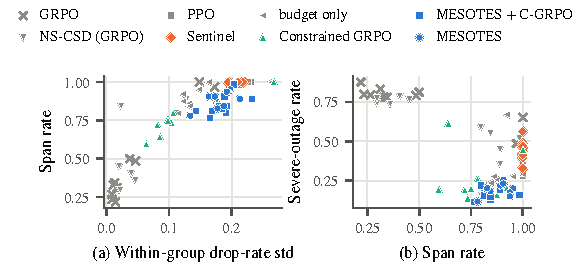
\includegraphics[width=\columnwidth]{figures/mechanism.pdf}
\caption{Evidence for constraint cancellation under full-intensity floods (80 trained checkpoints, $G=8$ members sharing common random numbers). (a)~The span rate increases with the within-group spread of the drop action. (b)~A lower span rate coincides with more severe outages. IMBANG restores both quantities.}
\label{fig:mech}
\end{figure}

% ===========================================================================
\section{The IMBANG Method}
\label{sec:method}
% ===========================================================================
\textbf{Safe-side member.} One member of every group is reserved. At each step it takes the policy's sampled action $(\tau,f,d)$, draws $u\sim\mathcal{U}(0.2,0.8)$ once per rollout, and executes
\begin{equation}
\tilde d=u\,d,\qquad \tilde\tau=\tau+(1-u)(1-\tau),\qquad \tilde f=f .
\label{eq:safe}
\end{equation}
\begin{proposition}[Monotone safety]\label{prop:safe}
For the same observation and traffic realisation, the collateral damage of the safe-side member after shielding never exceeds that of the policy member. Consequently, its number of severe outages is never larger.
\end{proposition}
\begin{proof}
By \eqref{eq:cd}, $\mathrm{CD}$ does not decrease with $d$, and it does not increase with $\tau$ because both $\alpha$ and $[\ell-C\tau]^+$ are non-increasing in $\tau$. The focus, and hence $\eta$, is left unchanged. Each shield rule is a per-coordinate $\min$ or $\max$ whose activation depends only on $(\mathbf{o}_t,f)$, so shielding preserves $\tilde d\le d$ and $\tilde\tau\ge\tau$. Finally, $\rho_t$ depends on the offered load and not on the action, so $\mathrm{SQ}=\rho(1-\mathrm{CD})$ inherits the ordering.
\end{proof}

Whenever the policy's samples cause outages that a less aggressive filter would avoid, the safe-side member can therefore supply the cost variation that Prop.~\ref{prop:cancel} shows to be necessary. The member influences the policy only through an advantage-weighted likelihood term, $-c\,[\hat A]^+\log\pi_\theta(\tilde a\,|\,\mathbf{o})$, so the policy moves towards it only when it outperformed the rest of its group. Monotonicity is a structural property that holds at every intensity and mutation level. IMBANG thus never needs to estimate where the outage threshold lies.

\textbf{Outage budget and model selection.} The multiplier is adjusted by dual ascent on the measured validation outage rate, $\lambda\leftarrow[\lambda+\eta_\lambda(\hat\sigma-\kappa)]^+$. The checkpoint that is deployed is chosen feasibility first: among checkpoints with $\hat\sigma\le\kappa$, the one with the highest validation score.

\textbf{Discrete minimax-regret levels.} In place of a learned attacker, training contexts are drawn from 360 discrete levels. These combine the attack family, six intensity bands, three mutation bands, pulsed or continuous flooding, and the presence of flash crowds, with ICMP excluded. Each level is scored by the MaxMC regret estimate~\cite{jiang2021robustplr}, $\mathrm{reg}(l)=\max_{k\le n}\hat J_k(l)-\hat J_n(l)$, computed with fixed common random numbers. Levels with high regret are revisited through prioritised level replay~\cite{jiang2021plr}.

\textbf{Common learner.} Every GRPO variant in this study uses the same learner. Each group of $G=8$ members holds policy samples, one archive elite, two shield probes and, for IMBANG, the safe-side member. The learner is anchored by a KL term to the best validated checkpoint and tunes the PanicGuard parameters under an empirical safety certificate. The network is Sentinel's two-layer, 64-unit architecture with Beta and categorical heads, trained without a critic. Algorithm~\ref{alg:span} outlines one iteration.

\begin{algorithm}[t]
\caption{One IMBANG training iteration}
\label{alg:span}
\small
\begin{algorithmic}[1]
\STATE Sample $B$ levels by MaxMC priority; warm up; fork each into $G$ members sharing one traffic realisation
\STATE Assign policy samples, elite, shield probes and the safe-side member \eqref{eq:safe}
\STATE Roll out $H$ windows through $\mathcal{S}_\phi$; form $R_g=O_g-\lambda K_g$ and group advantages $\hat A_g$
\STATE Update $\theta$: clipped surrogate on policy members, $[\hat A]^+$-weighted likelihood on the safe member and the elite, KL to the current champion
\STATE Every $K$ iterations: validate, update $\lambda$, select the champion feasibility first, and refresh MaxMC regrets
\end{algorithmic}
\end{algorithm}

% ===========================================================================
\section{Performance Evaluation}
\label{sec:eval}
% ===========================================================================
\textbf{Testbed fidelity.} We rewrote Sentinel's public simulator and shield~\cite{sentinelcode} as a batched implementation. Unit tests confirm that it agrees with the reference code to within $10^{-5}$. Re-running Sentinel's released benchmark checkpoints on this implementation recovers the published figures. For strong attacks, for example, we obtain quality, leakage and severe outages of 0.519, 0.815 and 78.2, compared with the reported 0.519, 0.815 and 75.0.

\textbf{Methods compared.} We compare the following defenders.
\begin{itemize}
\item \emph{Sentinel}: its released checkpoints for seeds 42--51.
\item \emph{PPO with shield}: an equal-budget baseline without co-evolution.
\item \emph{Constrained GRPO (C-GRPO)}~\cite{girgis2026cgrpo}.
\item Three minimal remedies applied on top of the same budget: no safe member, a six-fold entropy bonus, and an uncentred cost advantage in the spirit of~\cite{nie2026starvation}.
\item IMBANG.
\end{itemize}
All trained methods share Sentinel's network, use seeds 42--51 and receive roughly $1.35$M simulator steps; Sentinel's released run used $0.2$M co-evolution steps. The PPO baseline therefore serves as a compute-matched control (1.34M against 1.36M steps for IMBANG). It isolates how much of any improvement over Sentinel comes from the larger budget and the absence of co-evolution rather than from IMBANG itself.

\textbf{Protocols.} Protocol~B (attacker-agnostic) covers eight attack scenarios, four of them held-out stress tests, with 20 episodes of 100 windows each. Protocol~A replays, for each seed, the attacker that Sentinel trained alongside its defender; for IMBANG this is a transfer test. Protocol~C is a red team that runs a cross-entropy search over the whole scenario space, ICMP included, for the scenario that hurts each defender most. All comparisons are paired by seed and traffic realisation. We report paired $t$-tests with Holm correction together with Wilcoxon signed-rank tests.

\begin{table*}[t]
\centering
\caption{Attacker-agnostic Battery (Protocol B): Composite Score $\mathcal{B}$ ($\uparrow$), Severe Outages per 500 Steps ($\downarrow$) and Leakage ($\downarrow$), Mean over 10 Seeds}
\label{tab:main}
\setlength{\tabcolsep}{4.5pt}
\footnotesize
\begin{tabular}{@{}lccccccccc@{}}
\toprule
 & \multicolumn{3}{c}{Composite $\mathcal{B}$ ($\uparrow$)} & \multicolumn{3}{c}{Severe outages / 500 steps ($\downarrow$)} & \multicolumn{3}{c}{Attack leakage ($\downarrow$)} \\
\cmidrule(lr){2-4}\cmidrule(lr){5-7}\cmidrule(l){8-10}
Scenario & Sentinel~\cite{alfatemi2026sentinel} & C-GRPO~\cite{girgis2026cgrpo} & MESOTES & Sentinel & C-GRPO & MESOTES & Sentinel & C-GRPO & MESOTES \\
\midrule
Mild & 0.009 & \textbf{0.053} & 0.040\textsuperscript{\dag} & \textbf{0.0} & \textbf{0.0} & \textbf{0.0} & 0.983 & \textbf{0.917} & 0.941 \\
Strong & -0.746 & -0.612 & \textbf{-0.583}\textsuperscript{\dag} & 155.2 & 85.9 & \textbf{38.9} & 0.852 & \textbf{0.789} & 0.814 \\
Chaos/flash & -0.169 & \textbf{-0.114} & -0.123\textsuperscript{\dag} & 14.1 & 16.8 & \textbf{10.7} & 0.908 & \textbf{0.843} & 0.870 \\
ICMP (zero-shot) & -0.474 & -0.474 & \textbf{-0.458}\textsuperscript{\dag} & \textbf{4.6} & 23.3 & 18.0 & 0.748 & 0.727 & \textbf{0.716} \\
Pulsing$^\ast$ & -0.303 & -0.228 & \textbf{-0.225}\textsuperscript{\dag} & 60.5 & 37.7 & \textbf{16.1} & 0.877 & \textbf{0.825} & 0.847 \\
Polymorphic$^\ast$ & -0.454 & -0.442 & \textbf{-0.430}\textsuperscript{\dag} & 14.9 & 24.0 & \textbf{14.2} & 0.905 & \textbf{0.868} & 0.890 \\
Boundary-rate$^\ast$ & 0.003 & \textbf{0.084} & 0.071\textsuperscript{\dag} & \textbf{0.0} & \textbf{0.0} & \textbf{0.0} & 0.908 & \textbf{0.807} & 0.835 \\
ICMP-chaos$^\ast$ & -0.299 & \textbf{-0.255} & -0.257\textsuperscript{\dag} & 25.4 & 25.2 & \textbf{20.9} & 0.829 & \textbf{0.783} & 0.800 \\
\midrule
Mean$\pm$CI & -0.304$\pm$0.014 & -0.248$\pm$0.009 & -0.246$\pm$0.009 & 34.4$\pm$9.5 & 26.6$\pm$17.8 & 14.8$\pm$3.3 & 0.876$\pm$0.013 & 0.820$\pm$0.016 & 0.839$\pm$0.013 \\
\bottomrule
\end{tabular}

\vspace{2pt}
\parbox{\textwidth}{\scriptsize $^\ast$Held-out stress test (never used for training or model selection). Bold: best per metric. \dag\,MESOTES better than Sentinel (paired $t$-test over seeds, Holm-corrected across scenarios, $p<0.05$). Last row: mean $\pm$ 95\% $t$-interval over seeds of the scenario average.}
\end{table*}


\textbf{Comparison with Sentinel.} As Table~\ref{tab:main} shows, IMBANG achieves a significantly higher composite score than Sentinel in each of the eight attack scenarios after Holm correction. Averaged over scenarios, the scores are $-0.246$ and $-0.304$ ($p=1.2\times10^{-5}$). Severe outages fall from 34.4 to 14.8 per 500 windows ($p=0.002$) and leakage from 0.876 to 0.839 ($p<10^{-3}$), while service quality is unchanged (0.739 against 0.738, not significant). In five of the eight scenarios IMBANG is no worse than Sentinel on quality, leakage and outages simultaneously: strong, chaos/flash, pulsing, polymorphic and ICMP-chaos. When the traffic is generated by Sentinel's own trained attackers (Protocol~A), IMBANG still scores higher ($-0.265$ against $-0.332$, $p=0.019$) and lets less attack traffic through (0.778 against 0.830, $p=0.018$). The worst case uncovered by the red team improves from $-1.07$ to $-0.72$ ($p=7.2\times10^{-4}$).

\textbf{Is the gain due to the training budget?} Only in part. The compute-matched PPO baseline already improves on Sentinel ($-0.276$ against $-0.304$ in Protocol~B), which shows the benefit of dropping co-evolution and training on the operator's own score. IMBANG nevertheless beats this baseline at the same budget: $+0.030$ in Protocol~B ($p=2\times10^{-7}$) and $+0.050$ in Protocol~A ($p=0.011$), with less leakage in both (0.839 against 0.867, $p=0.002$). It also has fewer severe outages (14.8 against 19.6) and a better red-team worst case ($-0.72$ against $-0.79$), although these two differences are not significant.

\begin{figure}[t]
\centering
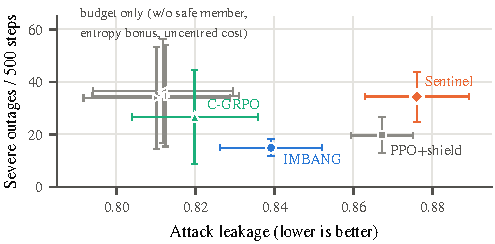
\includegraphics[width=\columnwidth]{figures/tradeoff.pdf}
\caption{Trade-off between severe outages and attack leakage (Protocol~B, averaged over the eight attack scenarios, with 95\% confidence intervals over ten seeds). Only IMBANG lowers both quantities relative to Sentinel.}
\label{fig:tradeoff}
\end{figure}

\begin{table}[t]
\centering
\caption{Ablation and Competitors (10 Seeds). B/A: Protocol B/A Composite; Sev.: Severe Outages per 500 Steps (B); Worst: Red-team Worst Case (C); Budget: Seeds Meeting the 5\% Validation Outage Budget; $\bar\lambda$: Final Multiplier}
\label{tab:ablation}
\setlength{\tabcolsep}{2.5pt}
\resizebox{\columnwidth}{!}{%
\begin{tabular}{@{}lcccccc@{}}
\toprule
Method & B $\uparrow$ & Sev. $\downarrow$ & A $\uparrow$ & Worst $\uparrow$ & Budget & $\bar\lambda$ \\
\midrule
Sentinel~\cite{alfatemi2026sentinel} & -0.304 & 34.4 & -0.332 & -1.07 & -- & -- \\
PPO + shield & -0.276 & 19.6 & -0.315 & -0.79 & -- & -- \\
GRPO (no budget) & -0.250 & 91.5 & -0.276 & -1.07 & -- & -- \\
\;+ MaxMC levels & -0.244 & 52.4 & -0.246 & -0.88 & 0/10 & 0.0 \\
\;+ budget & -0.253 & 36.5 & -0.248 & -0.87 & 1/10 & 7.7 \\
\;+ budget, entropy$\times$6 & -0.249 & 33.8 & -0.244 & -0.85 & 0/10 & 7.5 \\
\;+ budget, uncentred cost & -0.251 & 34.7 & -0.242 & -0.87 & 1/10 & 7.4 \\
\;+ budget, C-GRPO~\cite{girgis2026cgrpo} & -0.248 & 26.6 & -0.262 & -0.80 & 3/10 & 4.7 \\
\textbf{SPAN6G} (+ safe member) & -0.246 & 14.8 & -0.265 & -0.72 & 9/10 & 0.4 \\
SPAN6G + C-GRPO norm. & -0.247 & 12.1 & -0.266 & -0.71 & 7/10 & 0.4 \\
\bottomrule
\end{tabular}}
\end{table}


\textbf{Ablation and alternative remedies.} Table~\ref{tab:ablation} and Fig.~\ref{fig:tradeoff} separate the contribution of each ingredient.
\begin{itemize}
\item \emph{Plain GRPO} reaches a competitive score but causes 91.5 severe outages per 500 windows, which is the failure analysed in Section~\ref{sec:mechanism}.
\item \emph{A Lagrangian budget without the safe member} is satisfied in only one seed out of ten, even though the multiplier climbs to $\bar\lambda\approx7.7$. This matches Prop.~\ref{prop:cancel}: a larger $\lambda$ has no effect on groups whose members all violate the constraint.
\item \emph{An entropy bonus or an uncentred cost} does not restore feasibility either (zero and one seed respectively).
\item \emph{C-GRPO} meets the budget in three seeds.
\item \emph{IMBANG} meets it in nine, with a final multiplier of only $\bar\lambda\approx0.4$. Its composite score matches C-GRPO's ($p=0.47$), with higher quality ($+0.008$, $p=0.007$) and fewer outages (14.8 against 26.6), in exchange for slightly more leakage (0.839 against 0.820).
\item \emph{IMBANG with C-GRPO's channel-wise normalisation} lowers outages further to 12.1 (Wilcoxon $p=0.006$ against C-GRPO).
\end{itemize}
In overload conditions, the final IMBANG policies maintain a drop spread of 0.18 and a severe-outage rate of 0.19. Without the safe member, that rate is 0.35 (Fig.~\ref{fig:mech}).

\textbf{Deployment cost.} The deployed policy consists of the actor network and the rule-based shield. The actor has 5{,}447 parameters (21.8\,kB in 32-bit floating point) and needs about $5.3\times10^{3}$ multiply--accumulate operations per decision. On a single 2.1\,GHz Xeon core, one decision, including shielding, takes 0.24\,ms in PyTorch and 12\,$\mu$s as a plain NumPy forward pass. This is several orders of magnitude below the sub-second control windows of edge scrubbing, so the controller can run alongside the user-plane function or on a MEC host without dedicated accelerators. Training involves no extra inference cost at deployment: the safe-side member, the budget and the curriculum are used only in the digital twin.

\textbf{Limitations.}
\begin{itemize}
\item IMBANG does not surpass C-GRPO on the composite score; its advantage lies in reliably honouring the outage budget and in fewer outages.
\item Under zero-shot ICMP floods, IMBANG incurs more severe outages than Sentinel (18.0 against 4.6, not significant). A simulated operator playbook that reuses Sentinel's own ICMP constants removes the gap, with 2.1 severe windows at 90\% recognition accuracy.
\item On mild and boundary-rate floods, IMBANG gives up about 0.01 of service quality in return for 4--7 points less leakage.
\item Prop.~\ref{prop:safe} relies on congestion being evaluated on the offered load, as in Sentinel's simulator.
\item All results are simulation-based; replaying real traces such as 5G-NIDD remains future work.
\end{itemize}

% ===========================================================================
\section{Conclusion}
% ===========================================================================
Training a neuro-symbolic DDoS defender with critic-free group-relative updates does away with the value network and the adversarial training loop. The price is that any safety cost borne by a whole group silently disappears from the update. IMBANG restores that cost with a single safe-side member per group, constructed from a monotone safety direction guaranteed by the service model. The resulting defender outperforms the co-evolutionary Sentinel in every attack scenario of an attacker-agnostic benchmark and more than halves its severe outages. It also meets an operator outage budget far more consistently than Constrained GRPO, and it beats a compute-matched PPO baseline. With 5.4k parameters and sub-millisecond decisions, it is light enough for deployment at the edge. Validating IMBANG on replayed real traffic is the next step. The source code, configurations and per-seed results accompany this paper.

\bibliographystyle{IEEEtran}
\bibliography{refs}

\end{document}
